\subsubsection*{Validación de supuestos}
En esta sección comprobaremos que los supuestos necesarios para utilizar la regresión lineal sean o no válidos para los modelos que nos interesan, estos son: M2 y M4
\vskip0.2cm\textbf{Modelo 2}
\begin{itemize}
    \item \textbf{Homocedasticidad}: comprobaremos los supuestos de homocedasticidad graficando $t_i$ vs $\hat{y}_i$
    \begin{figure}[H]
        \centering
        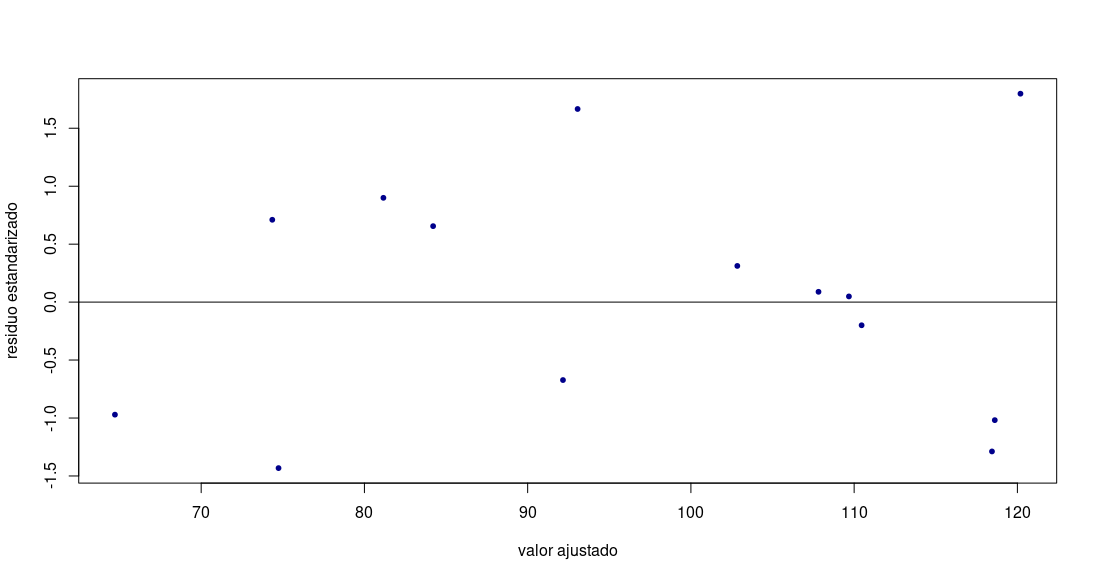
\includegraphics[width=0.7\textwidth]{resources/supuestos_M2.png}
        \caption{Homocedasticidad: modelo 2}
    \end{figure}
    Podemos ver que si bien no aparenta haber una relación de dependencia entre los valores estimados y los residuos, creemos que es difícil obtener esta información con pocas muestras.
    \item \textbf{Normalidad}:
    graficamos un qq-norm para los residuos.
    \begin{figure}[H]
        \centering
        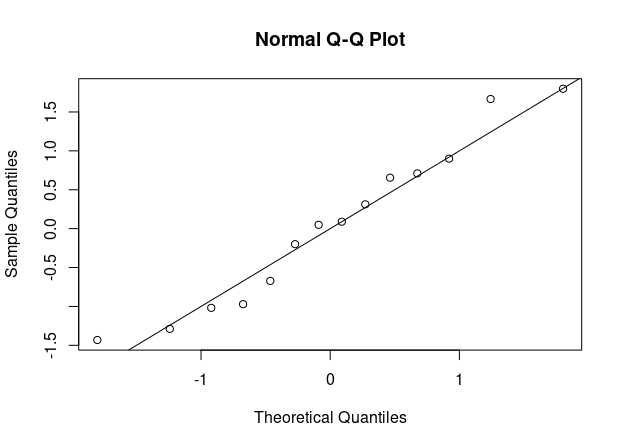
\includegraphics[width=0.7\textwidth]{resources/normalidad_m2.png}
        \caption{Normalidad: modelo 2}
    \end{figure}
    Era de esperarse que estos se distribuyeran aproximadamente como una t de student, y viendo el gráfico no encontramos evidencia suficiente para rechazar dicho supuesto.
\end{itemize}

\vskip0.2cm\textbf{Modelo 4}
\begin{itemize}
    \item \textbf{Homocedasticidad}: comprobaremos los supuestos de homocedasticidad graficando $t_i$ vs $\hat{y}_i$
    \begin{figure}[H]
        \centering
        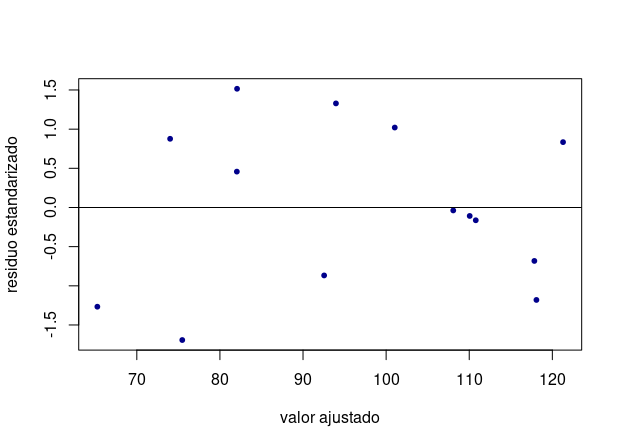
\includegraphics[width=0.7\textwidth]{resources/supuestos_M4.png}
        \caption{Homocedasticidad: modelo 4}
    \end{figure}
    Igual que antes, parece no aparentar ningún tipo de relación muy marcada entre los valores ajustados y los residuos. De todas formas en este caso tampoco tenemos las muestras suficientes como para afirmar o rechazar esta idea.

    \item \textbf{Normalidad}:
    Graficamos un qq-norm para los residuos.
    \begin{figure}[H]
        \centering
        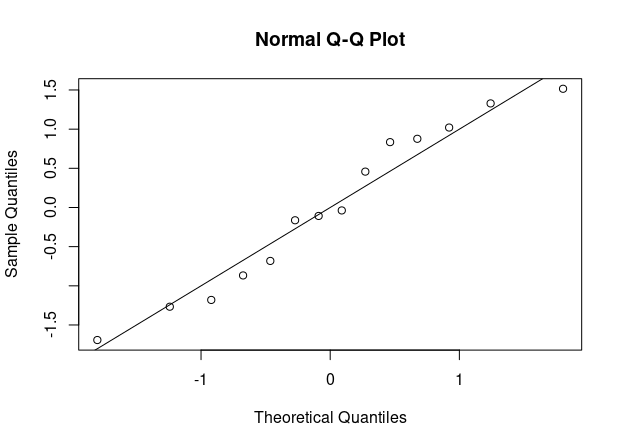
\includegraphics[width=0.7\textwidth]{resources/normalidad_m4.png}
        \caption{Normalidad: modelo 4}
    \end{figure}
    Nuevamente los residuos se distribuyen como esperábamos, esto es: de forma simétrica, similar a una normal pero con las colas pesadas. A diferencia del caso anterior se notan leves protuberancias en los valores intermedios pero no son suficientemente significantes como para decir que no se sigue dicha distribución.
\end{itemize}

\subsubsection*{Gráficos extra}
A continuación graficaremos para el modelo 4 como se ve su estimación en 3 dimensiones.
\begin{figure}[h]
    \centering
    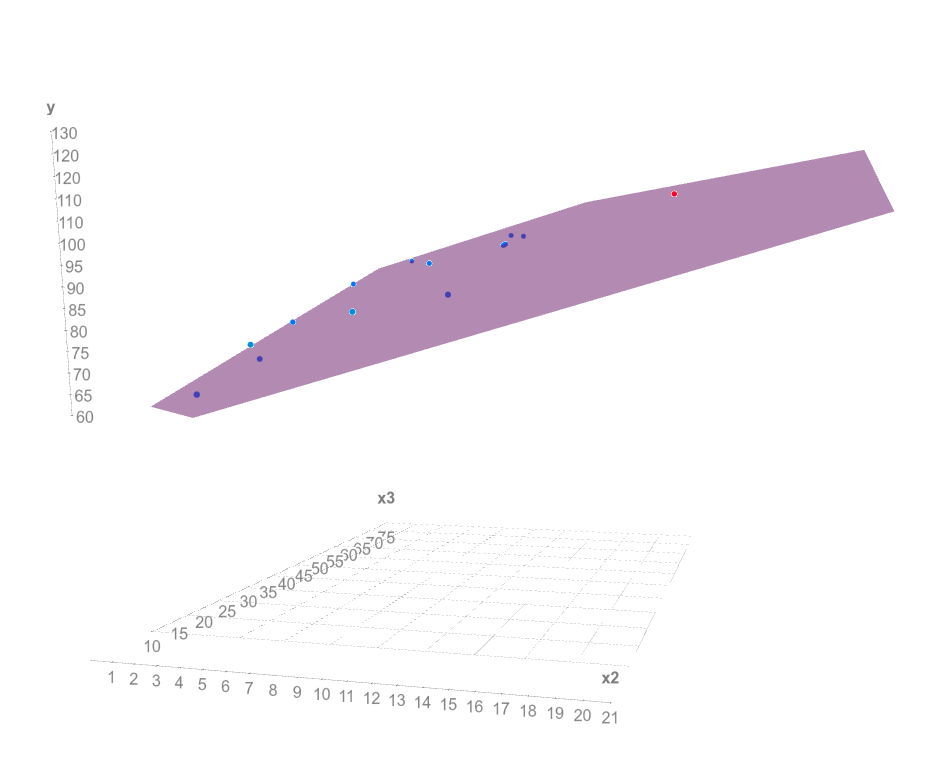
\includegraphics[width=0.8\textwidth]{resources/prediccion_m4.png}
    \caption{Estimación del modelo 4}
\end{figure}

Podemos ver que efectivamente el modelo parece ajustar a las muestras, y parece predecir correctamente.\\
Mostramos en rojo al valor atípico identificado para $X_2$ en la sección 1.

\subsection*{Transformación Box-Cox}
Queremos observar qué sucede si a nuestro modelo 4 le aplicamos una transformación Box-Cox, por lo que primero buscaremos el $\lambda$ de máxima verosimilitud.

\begin{minipage}{\linewidth}
  \begin{minipage}{0.45\linewidth}
    \begin{figure}[H]
        \centering
        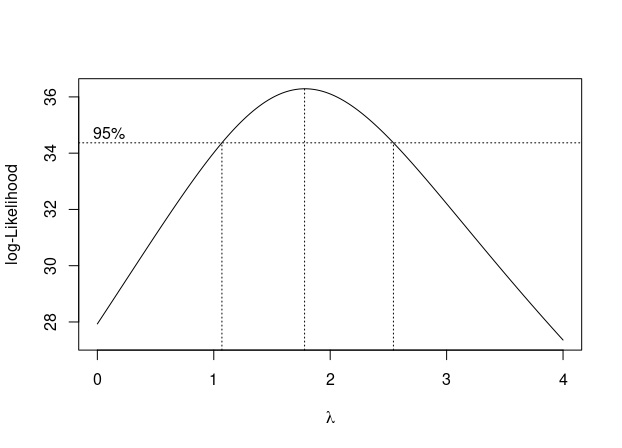
\includegraphics[width=1\textwidth]{resources/lambda_mv.png}
        \caption{Estimación de $\lambda$}
    \end{figure}
  \end{minipage} 
  \begin{minipage}{0.45\linewidth}
    En este gráfico podemos ver:
    \begin{enumerate}
        \item Un intervalo de confianza del $95\%$ para el parámetro $\lambda$, este se mueve en torno al intervalo $[1.1; 2.5]$
        \item El estimador de máxima verosimilitud de $\lambda$ se encuentra en el valor: $1.78$
        \item El valor de $\lambda = 2$ se encuentra dentro del intervalo de confianza del $95\%$
    \end{enumerate}
  \end{minipage}
\end{minipage}

\vskip0.2cm

Para la transformación decidimos utilizar $\lambda = 2$, por lo que, ahora deberíamos regresar el siguiente modelo:
$$
Y^{(2)} = \frac{Y^2 - 1}{2} = \beta_0 + \beta_1 X_2 + \beta_2 X_3
$$
\vskip0.2cm
La regresión que obtuvimos fue la siguiente:
$$\frac{Y^2 - 1}{2} = 614.2  + 167.87 X_2 + 66.14 X_3$$ que es 
equivalente a:
$$Y = \sqrt{1229.4 + 335.74 X_2 + 132.28 X_3}$$

El nuevo modelo planteado obtuvo un error cuadrático medio estimado de $4.02$ que es el mejor de todos.
A continuación mostraremos un gráfico del ajuste propuesto:

\begin{figure}[H]
    \centering
    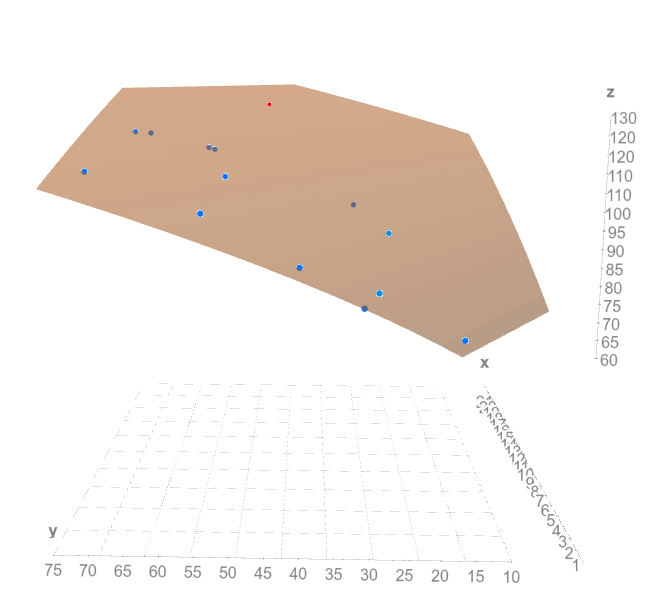
\includegraphics[width=0.7\textwidth]{resources/prediccionfacha.png}
    \caption{Ajuste del modelo transformado}
\end{figure}